% To do:
% ------
% - Write an outline.
% - Fill in the outline.
% - Publish on the arXiv.
% - format for ICML Position Paper and submit.
% - Wait for the call from Stockholm.

% Style notes:
% ------------
% - Be very careful about the SUBJECT of sentences. Is it ML that is bad? Is it the practice that is bad? Is it the practitioner that is bad?
% - [more here]

\documentclass[11pt]{article}
\usepackage[utf8]{inputenc}
\usepackage{microtype}
\usepackage[letterpaper]{geometry}
\usepackage{xcolor}
\usepackage{graphicx}

% Hogg typesetting issues
\setlength{\textwidth}{6.00in}
\setlength{\oddsidemargin}{0.25in}
\setlength{\oddsidemargin}{0.00in}
\setlength{\textheight}{9.25in}
\setlength{\topmargin}{-0.50in}
\setlength{\parindent}{1.2\baselineskip} % seriously
\renewcommand{\title}[1]{\section*{\raggedright #1}}
\renewcommand{\author}[1]{\medskip\par\noindent\textbf{#1}}
\newcommand{\affil}[1]{{\footnotesize\par\noindent #1 \par}}
\renewenvironment{abstract}{\paragraph{Abstract:}}{}
\newcommand{\documentname}{\textsl{Position Paper}}
\newcommand{\sectionname}{Section}
\newenvironment{hoggnumerate}
  {\begin{list}
    {\arabic{enumii}.}
    {\usecounter{enumii}
     %\setlength{\labelwidth}{3em}
     %\setlength{\labelsep}{0em}
     \setlength{\itemsep}{0in}
     \setlength{\parsep}{0in}
     \setlength{\parskip}{0in}
     %\setlength{\leftmargin}{1.5cm}
     %\setlength{\rightmargin}{2cm}
     %\setlength{\itemindent}{0em} 
     %\let\makelabel=\makeboxlabel
    }
  }
{\end{list}}
\pagestyle{myheadings}
\markboth{foo}{\textcolor{gray}{\textsf{Hogg / Is machine learning good or bad for the natural sciences?}}}
\linespread{1.08}
\frenchspacing\raggedbottom\sloppy\sloppypar

% Gross
\newcommand{\apj}{The Astrophysical Journal}
\newcommand{\araa}{Annual Reviews in Astronomy and Astrophysics}

% Math issues
\newcommand{\teff}{T_{\mathrm{eff}}}
\newcommand{\logg}{\log g}
\newcommand{\feh}{[\mathrm{Fe}/\mathrm{H}]}

\begin{document}\thispagestyle{empty}

\title{\documentname: Is machine learning good or bad for the natural sciences?}

\author{David W. Hogg}
\affil{Center for Cosmology and Particle Physics, Department of Physics, New York University, 726~Broadway, New~York,~NY 10003, USA}
\affil{Center for Data Science, New York University, 60 Fifth Avenue, New York, NY 10011, USA}
\affil{Max-Planck-Institut f{\"u}r Astronomie, K{\"o}nigstuhl 17, D-69117 Heidelberg, Germany}
\affil{Flatiron Institute, a division of the Simons Foundation, 162 Fifth Avenue, New~York,~NY 10010, USA}

\begin{abstract}
  Machine learning (ML) methods are having a huge impact across all of the sciences.
  However, ML has a strong ontology---in which only the data exist---and a strong epistemology---in which a model is considered good if it performs well on held-out training data.
  These philosophies are in strong conflict with both standard practices and key philosophies in the natural sciences.
  Here we identify locations for ML in the natural sciences where the ontology and epistemology are valuable.
  For example, when a flexible machine-learning model is used in a causal inference to represent the effects of confounders, such as foregrounds, backgrounds, or instrument calibration parameters, the model capacity and loose philosophy of ML can sometimes make the results more trustworthy.
  We also show that the there are contexts in which the introduction of ML introduces strong, unwanted statistical biases.
  For one, when flexible models are used to emulate physical (or first-principles) simulations, they introduce strong confirmation biases.
  For another, when flexible regressions are used to make datasets, the elements of those datasets cannot be used in joint analyses without taking on uncontrolled biases.
  These remarks are intended to apply to all of the natural sciences, but most of the specific examples are in the astrophysics domain.
\end{abstract}

\section{Introduction}\label{sec:intro}
It is an understatement to say that machine learning (ML) is having a big impact across the sciences.
A significant fraction of all scientific papers in the natural sciences now employ ML in part (or all) of their analyses.
However, when we ask what scientific breakthroughs have been enabled by this influx of new tools and methods, there isn't a long list.
The success of the AlphaFold projects in protein structure \cite{alphafold} are often raised.
But these are successes in a very specific challenge-problem setting in which \emph{performance} is valued over \emph{understanding}.
In the natural sciences we almost exclusively care about understanding, in the long run.

The natural sciences are concerned with understanding the world, and naturally occurring mechanisms in play in that world.
We make progress by discovering new kinds of objects and phenomena, and explaining (and, even better, predicting) qualitatively new kinds of objects and phenomena.
Our most successful investigations are judged in terms of the questions they answer, or the new questions they raise, or both.
The question here is: How will ML contribute to this mission?

In contrast to natural science, ML research and ML methods are concerned with making accurate predictions for, or descriptions of, \emph{data}.
A ML method is considered successful if it performs well on held-out training data, even if the latent structure of the model is generic and the internals are impossible to interpret.
In ML, the considerations are all at the level of the data, and we are happy to use models where we have litlle or no understanding of the meanings or values of the latent parameters or weights.
Another way to ask our question is:
\emph{Where, in the natural sciences, can you use a model that you don't understand?}

In natural science the most important contributions and results are all at the level of the \emph{latents}:
We use data to learn about the latent structure of the world or of the system we are studying.
In astrophysics, this could be the interior structure of the Sun, or the statistics of planets around other stars, or the map of the dark matter surrounding the Milky Way.
The things we care about are almost never directly observable; they are parameters (or hyper-parameters) of a physical (or chemical or biological) model that predicts the observables.

For a concrete example, when the expansion of the Universe was discovered \cite{expansion, expansion2}, the discovery was important, but not because it permitted us to predict the values of the redshifts of new galaxies (though it did indeed permit that).
The discovery was important because it told us previously unknown things about the age and evolution of the Universe, and it confirmed a prediction of general relativity, which is a theory of the latent structure of space and time.
The discovery would not have been seen as important if Hubble and Humason had instead announced that they had trained a deep multilayer perceptron that could predict the Doppler shifts of held-out extragalactic nebulae.

We are both ML \emph{skeptics} and ML \emph{practitioners}.
We are writing this for an audience that is either developing an ML method for science applications or else bringing ML into a scientific domain.
The main points of this \documentname{} are \textsl{(1)}~that ML has places where it is very valuable in the contemporary practice of science, and \textsl{(2)}~that it also has places where it will create problems for science.
The answer to the question in the title is ``Both.''

\paragraph{Our contributions:}
\begin{itemize}
  \item We deliver a description of the fundamental \emph{ontology} and \emph{epistemology} of machine learning, and contrast these with the ontologies and epistemologies of the natural sciences.
  \item We elucidate two important and strong statistical biases that are being introduced to the natural sciences by some of the uses of ML in those disciplines. One is a confirmation bias that arises when simulations are replaced or augmented by emulators. Another is a more standard estimator bias that is (possibly enormously) amplified when elements of datasets produced by ML regressions are used in combination or joint analyses.
  \item We show that there are many safe places for the use of ML methods in current natural-science practices, and places where (in the contemporary context) the use of ML methods is effectively \emph{required}. Many of these places are in the operational parts of scientific projects.
  \item Further, we demonstrate that there are contexts inside a natural-scientific analysis in which using the most flexible ML method delivers \emph{the most conservative approach} to the scientific problem. An example is in causal contexts, where providing immense flexibility to (say) a confounder model can strengthen conclusions about the causal channels of interest.
\end{itemize}

\section{The ontology and epistemology of machine learning}\label{sec:philosophy}

\paragraph{What is machine learning?}
For the purposes of this \documentname, we will employ an expansive or inclusive definition of ML.
For us, a method is ML if its \emph{capability increases substantially as it sees more data} \cite{ml_definition}.
In some sense this definition could be seen as true of any measurement process, since measurements improve as the data improve. 
If we are going to be more specific, we'd like the model precision or capability to improve faster (in some sense) than (something like) the square root of the increment in data.

This definition is broad:
In addition to methods like convolutional neural networks \cite{cnn}, multi-layer perceptrons \cite{mlp}, and transformers \cite{transformer}, it includes large linear regressions \cite{linearregression}, gaussian processes \cite{gp}, support-vector machines \cite{svm}, principal components analysis \cite{pca}, kernel density estimates \cite{kde}, and even some kinds of multilayer or hierarchical models \cite{multilevel}.
Feel free to personally take any more restrictive definition.
Our comments will apply to everything in the larger class.

\paragraph{Ontology:}
Unsupervised ML methods deliver descriptions or compressions of data.
Supervised ML methods find relationships between data (features) and data (labels).
In both cases, the methods are judged on their capability to accurately describe the data.
They are not judged on the details of their latent structure.
In a very important sense, the ML ontology is that \emph{only the data exist}.

In support of this point of view, here are some comments:
Deep-learning models have enormously large internal degeneracies (combinatorial degeneracies even).
These degeneracies are not seen as a problem, since all they do is make the latent weights less interpretable.
Contemporary optimization schemes are stochastic \cite{stochastic} and most models are non-convex.
The fact that it is impossible to find the global optimum---and the fact that in most contemporary models that isn't even the goal \cite{not_global}---shows that the latent parameters are not important.
The use of early stopping \cite{early_stop} and drop-outs \cite{dropout} to stabilize optimization strengthens this point.
Any practitioner using a 40-layer network can trivially (and without analysis) switch to a 42-layer, despite the fact that (from a functional point of view), this substantially changes the model capacity.

Models are deemed stably optimized and useful not if the latent space is stable, but rather if the predictions for held-out data are stable.
Thus it is the data that exist in ML contexts, not the latent parameters.

\paragraph{Epistemology:}
A trained ML model is deemed successful or correct if \emph{it performs well on held-out training data}.
This epistemological position is related strongly to the ontological position:
If only the data exist, then the success of a model is judged only in terms of the data it describes.

In support of this position we could point to the literature on adversarial attacks \cite{adversarial1, adversarial2}.
This literature shows us, in dramatic ways, that ML methods are not doing what we (na\"ively) believe that humans or scientists or scientific theories do in comparable circumstances.
And yet, these attacks do not suggest (to most practitioners of ML) that the methods are wrong or require revision.
Even the responses to attacks have responded in ways that involve augmentation of data \cite{adversarial_training}, such that the vulnerability to attack is lessened without compromising the fundamental epistemological point that performance on data is the primary standard of truth.

A critic of our epistemological claim could point to the large literature on out-of-sample generalization, transfer learning \cite{transfer}, or the more grand contemporary idea of foundation models \cite{foundation}.
But even in these contexts, models are deemed successful when they explain new or held-out data; the latent structure of the models is not a primary consideration when the validity of the model is in question.

\paragraph{Natural sciences:}
Ontologies and epistemologies are somewhat different in different scientific fields---and among different practitioners---but in almost no natural-scientific context do the ontology and epistemology match those of ML.

In physics, for example, the ontology is much broader than it is in ML.
Not only do the data exist, but so do forces, energies, momenta, charges, spacetime, wave functions, virtual particles, and much more.
These entities are judged to exist in part because they are involved in the latent structure of the successful theories; almost none of them are direct observables.

In physics the epistemology is much more restrictive than it is in ML.
A physics model---which, as we note, is almost always a model of latent structure---is judged to be good or strongly confirmed if it explains some aspects of different data in multiple domains, and if it connects in natural ways to other theories or principles (such as conservation laws and invariances) that are strongly confirmed themselves.
It is worthy of note here that a successful theory is usually a combination of a simple theory of the latents, and a less simple observation model, which explains how the latents appear in the data space.

HOGG: DROP THIS? Differences aside, there is an argument to make that maybe the natural sciences could be better off if they moved at least slightly closer to the ML points of view on ontology and epistemology.
In the long run, the data are more stable than the fundamental theories of physics:
Newtonian gravity was replaced with general relativity, and we expect general relativity to be replaced by some kind of quantum gravitational theory.
At each change, the ontology changes, while the data are stable.
We are not recommending this, but noting that a robust philosophy of science might be more positively oriented towards the data than standard practice.

\section{Why do we need machine learning in the natural sciences?}
In this \sectionname{} we give some idea of how and why ML has had such a big impact in the natural sciences, and how and why many scientific projects require ML technologies.
In most cases, the ML is required on the engineering or execution side of projects that are large-scale in some sense.
\begin{description}
  \item[Label transfer:] Sometimes a project has informative data on a very large number of objects, but precise labels for only a few, maybe obtained through very careful analysis or external data.
  In this case, if it is extremely expensive to label more objects, a regression can be trained on the labeled data points and then the trained regression used to label
  \item[Classification:]
  \item[Speeding up decisions:]
  \item[Speeding up simulations:]
  \item[Modeling nuisances:]
  \item[Outlier detection:]
  \item[Making discoveries?]
\end{description}
The short summary is that we need ML in the natural sciences; we can't live without it.
The question here is how we will use it safely?

\section{When is machine learning bad for natural science?}\label{sec:bad}
In this \sectionname{} we elucidate two statistical biases that can be introduced when ML methods are introduced into a natural-science project.
Neither of these biases can be easily corrected or removed.

\paragraph{Amplifications of training-set biases:}
The outcomes of ML regressions are label estimates that are conditioned on the input features \emph{and also} on the totality of the training set used to train the regression.
This is good; the individual-data-point label estimates from the regression are the lowest ``risk'' (in the statistical sense) when they use non-zero bias in the bias--variance trade-off.
However, the biases that are weak or manageable on an individual data-point basis become strong or unacceptable biases when outputs of regressions are used jointly or in combination to measure a population or sub-population property.

This problem is demonstrated with a toy example in \appendixname~\ref{app:toy}.
It is worst when the regression is used to label a large data set or catalog or sample of data,
and when elements of that data set are used in populations or joint analyses.
In general, when multiple data point estimates are used jointly, the variance-induced offsets of the estimators average out but the bias-induced offsets remain fixed.
This is a straightforward point of statistics---this is not news---but it isn't currently informing most of the practice of ML in the natural sciences.
For example, HOGG CITES.

In principle, there are fixes for this problem that involve de-biasing the estimates.
This is not possible in general, because there is not usually enough validation data to accurately assess the bias.

In Bayesian language, this problem is closely related to the point that when data are to be combined, they should be combined at the likelihood level, not the posterior level.
Likelihoods are not affected by population-level biases, and potentially produce unbiased estimates.
Likelihood-based estimators are not usually the lowest-risk estimators, but they can be low- or zero-bias estimates.
The outputs of regressions are more like posterior-based estimators, affected by the implicit prior set by the training set.
When they are combined, the implicit prior gets amplified.
Most ML regressions are not capable of generating or emulating likelihoods.
There are interesting approaches in development to replace regressions with generative models that can produce likelihoods HOGG CITE THINGS.

Finally we note---and demonstrate in \appendixname~\ref{app:toy}---that none of these problems arise from out-of-sample generalization or distribution-shift problems.
Distribution shifts just tend to make these kinds of problems worse.

\paragraph{Emulator-induced confirmation bias:}
In many fields in the natural sciences, the fundamental theoretical model is \emph{computational}, meaning that theoretical predictions are made with large computer simulations.
These simulations are usually limited in the range of length scales and time scales which they can simultaneously compute.
Comparison of data with simulations usually involves running enormous numbers of simulations \cite{sbi}, because simulations have to span ranges of fundamental parameters and initial conditions and so on.
Thus these simulation requirements are getting very large for contemporary research projects.
For example, in cosmology contemporary experiments could easily consume the total computing capacity of the United States.
Hence we turn to emulators---trained ML regressions that have learned the input-output relationship of a simulation, or the relationship between an inexpensive low-resolution simulation and an expensive high-resolution experiment.
Emulators can make computationally impossible projects possible.

Recall that because these emulators are ML methods, they generally have uninterpretable internal parameters and weights, and they generally have been validated by comparison with held-out training data.
Like all high-capacity ML methods, they generally are vulnerable to adversarial attacks.

Now imagine that two cosmology experiments proceed to do enormous emulator-based inferences on large data sets.
Imagine that these inferences are so large that it would have been exceedingly expensive to have done them with the original first-principles simulations instead of the emulators.
Experiment A finds cosmological parameters very much in line with our expectations going in.
Experiment B finds something extremely surprising about the mass matrix for the neutrinos, in conflict with other measurements and our expectations.
The comment is made, when the results of Experiment B come out, that perhaps the anomaly comes from something very slightly wrong or off in the trained ML emulator.

By construction, both experiments are extremely expensive to re-analyze with first-principles simulations.
Which one would we fund for reproduction?
The motivation to re-analyze Experiment B is far, far higher than the motivation to re-analyze Experiment A.
That is a classic example of \emph{confirmation bias}.

Since the money involved is astronomical, there is no simple fix for this unless we plan to re-analyze all experiments using first-principles simulations, no matter what they find.
If that is what's required to avoid the bias, then we should just analyze everything with simulations in the first place, and never use the emulators at any stage.

\section{When is machine learning good for natural science?}\label{sec:good}

\paragraph{Foreground, background, and confounder models:}

\paragraph{Outlier detection:}

\section{Discussion}\label{sec:discussion}

Hello World!

\paragraph{Acknowledgements:}
It is a pleasure to thank
  Gaby Contardo (SISSA),
  Jennifer Hill (NYU),
  Adrian Price-Whelan (Flatiron),
  Sam Roweis (deceased),
  Bernhard Sch\"olkopf (MPI-IS), and
  Soledad Villar (JHU)
for conversations over the years related to these arguments.

{\raggedright
\bibliography{ml_in_astro}
\bibliographystyle{plain}
}

\clearpage\appendix
\section{Population-level biases in regression outputs}\label{app:toy}
A machine-learning (ML) regression learns the best set of parameters (weights and thresholds, for example) $\hat{\theta}$ of a flexible function $f(x;\theta)$ from a training set of labeled data.
The learned function $f(x;\hat{\theta})$ delivers a predicted or estimated label $\hat{y}$ for any data point with a complete set of features $x$.
Thus an estimated label $\hat{y}_\ast$ for a data point with features $x_\ast$ has taken information \emph{both} from the features $x_\ast$ and \emph{also} from the features and labels of all the data points in the training set used to set the parameters $\hat{\theta}$.
In applications in which regression-estimated labels are used, it matters \emph{how much information} is coming from the individual data-point's features and how much from the original training set.

To illustrate these ideas, we construct a toy data analysis.
This toy will make a general point, but it has a decidedly astronomical feel to it.
The complete toy data set is generated by a process with the algorithm below.
This algorithm makes references to objects $\xi_\eta$ and $\xi_\zeta$ which are generated prior to the start.
\begin{hoggnumerate}
    \item A floating-point value of a known parameter called ``guiding radius'' $r$ is generated in the range $0<r<14$.
    \item A floating-point value of a latent parameter called ``age'' $\eta$ is generated from a Gaussian with mean $14 - r$ and variance 4.
    \item The point is discarded if the age is outside the range $0<\eta<13$. If the point is not discarded:
    \item A $K$-dimensional latent vector $\zeta$ with $K=14$ is generated from a Gaussian with zero mean and variance 1.
    \item A $M$-dimensional latent vector $\xi$ with $M=110$ is created by $\xi = \xi_\eta\,\eta + \xi_\zeta\cdot\zeta$, where $\xi_\eta$ is a $M$-vector and $\xi_\zeta$ is a $M\times K$ matrix.
    The elements of $\xi_\eta$ and $\xi_\zeta$ were drawn (before the start) from Gaussians with zero mean and variances $0.01/K$ and $1/K$ respectively.
    \item A rectified latent vector $\tilde{\xi}$ is created by taking $1 + \xi$ and rectifying all pixels to lie in the range $[0, 1]$.
    \item A $M$-dimensional feature vector $x$ called ``the data'' is generated from a Gaussian with mean $\tilde{\xi}$ and variance $0.0025$.
    \item A label $y$ called ``measured age'' is generated from a Gaussian with mean $\eta$ and variance 1.
\end{hoggnumerate}
The data generated this way are shown in the top panels of \figurename~\ref{fig:regression}.
The data contain a non-trivial relationship between label $y$ (measured age) $y$ and known parameter $r$ (guiding radius).
This relationship is shown in \figurename~\ref{fig:regression}.
It isn't precisely linear because of the censoring of data points with latent ages outside the range $0<\eta<13$.

We construct a three-layer multilayer perceptron (MLP) (using the scikit-learn implementation) with layer sizes of 64, 32, and 16 neurons.
The model is trained on a training set of 4096 data points with features $x$ and labels $y$.
The trained model takes as input features $x$ and outputs estimated labels $\hat{y}$.
The model is validated on a validation set of 2048 data points with features $x$ and labels $y$.
The test set is a much larger set of 105,864 data points with features $x$ and no labels.
The model is used to make estimated labels $\hat{y}$ in the full test set.
The validation and test labels are shown in the bottom panels of \figurename~\ref{fig:regression}.
Importantly, \emph{the training, validation, and test samples are drawn from exactly the same process}, with the same distribution in all properties.
\begin{figure}[p!]
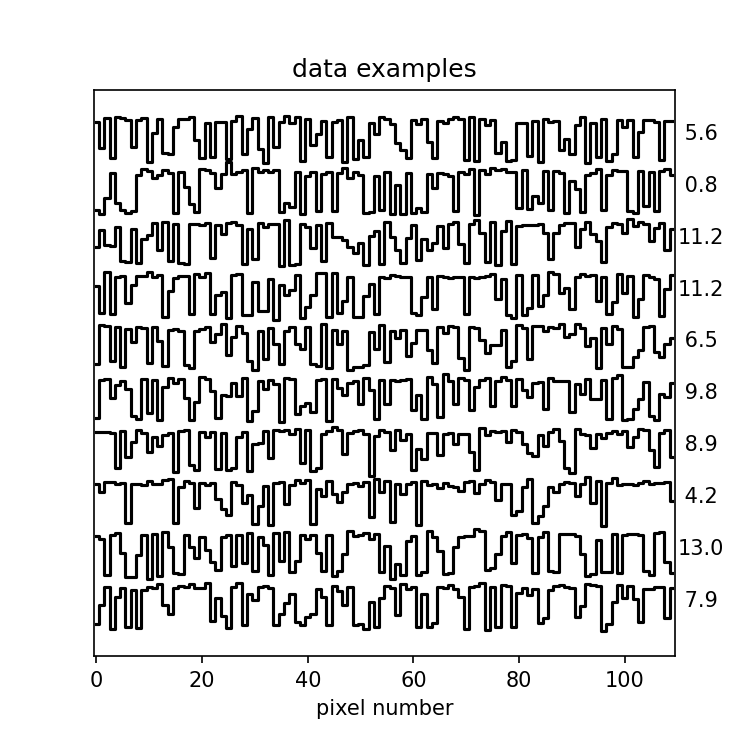
\includegraphics[width=0.49\textwidth]{notebooks/data_examples.png}
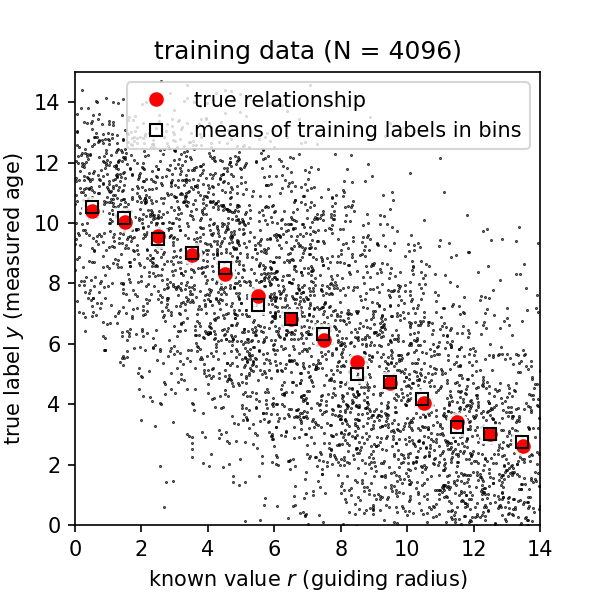
\includegraphics[width=0.49\textwidth]{notebooks/training_data.png} \\
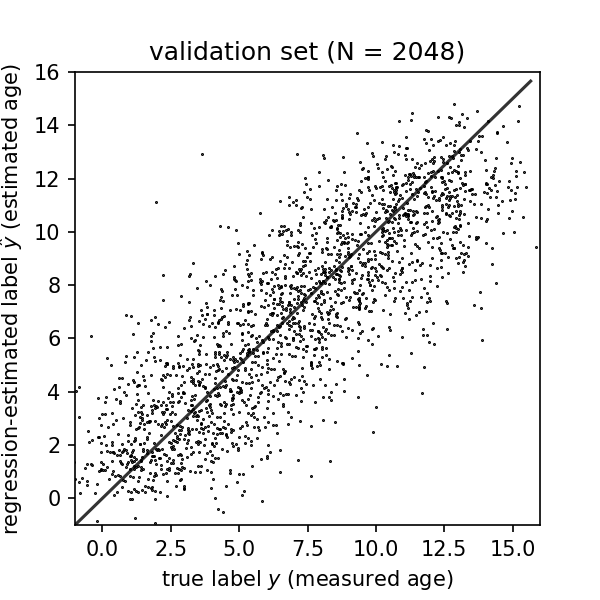
\includegraphics[width=0.49\textwidth]{notebooks/validation.png}
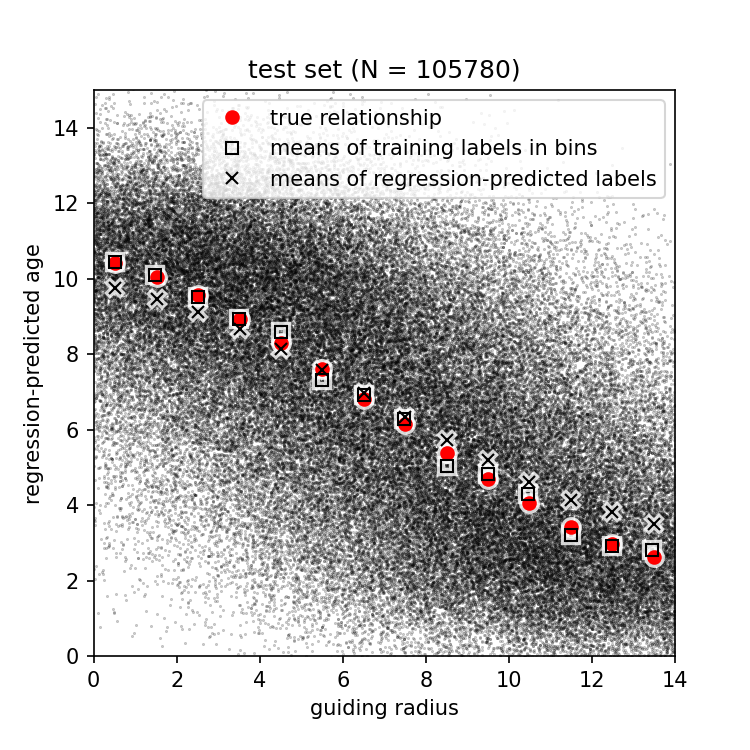
\includegraphics[width=0.49\textwidth]{notebooks/test_data_results.png}
\caption{\sffamily%
Visualization of the toy regression. \textsl{Top-left:} Random examples of the data vectors $x$, which are one-dimensional images generated from a linear model plus a nonlinearity created by two rectifications. Details of the data generation are given in the text. Each example $x$ is labeled on the right side by the value of its label $y$. \textsl{Top-right:} The training-set labels $y$, plotted against the known parameter $r$, which is not used in the regression (only the vectors $x$ are used). Also shown are solid red circles showing the true mean relationship between $y$ and $r$ in the toy data. Open black squares show the empirical mean relationship measured in bins in the training-set data. \textsl{Bottom-left:} Validation of the trained regression in the validation set, showing that the label estimates $\hat{y}$ are noisy (as expected given the problem set-up) but not strongly biased. \textsl{Bottom-right:} The regression estimates $\hat{y}$ in the very large test set, plotted against the known parameter $r$. Also shown are the same solid red circles and open black squares as in the top-right plot. Black exes show the mean relationship between $\hat{y}$ and $r$. The relationship shown by the exes is very precise but biased far away from the true relationship, unlike the relationship shown by the open squares (measured in the training set alone).\label{fig:regression}}
\end{figure}

The regression-estimated labels $\hat{y}$ are related to the measured labels $y$ in the validation set with a linear relationship with unit slope and zero intercept.
They are not precisely estimated, but there is no evidence for bias at the individual-object level.

The true relationship between label $y$ (measured age) and known parameter $r$ (guiding radius) is estimated in a large generated data set by taking means of $y$ in bins of $r$.
This relationship is shown in \figurename~\ref{fig:regression} with solid red circles.
The empirical relationship between label $y$ and known parameter $r$ in the training-set data is shown in \figurename~\ref{fig:regression} with open black squares.
These two relationships are statistically consistent.
The empirical relationship in the test-set data between the estimated label $\hat{y}$ and the known parameter $r$ in the test-set data is shown in \figurename~\ref{fig:regression} with black exes.
The test-set relationship is strongly biased, deviating from the true relationship at the edges of the $r$ range.
Given the large size of the test set, the precision of the result is high: This bias in the estimated relationship is larger than 30-sigma in the worst data points.

HOGG: What to do? Just use the training set!

HOGG: Note that none of these problems come from bad data, out-of-distribution, or complexity.

HOGG: Link to notebook / github.

\end{document}
